\chapter{Anomaly Detection and Ensemble Learning: a Review} \label{chap:sota}

\section*{}

The chapter introduces the main concepts in this thesis: \textit{Anomaly Detection} and \textit{Ensemble Learning}. Definitions will be provided for both, along with a taxonomy for the approaches used in each. Finally, the state-of-the-art of Ensemble Learning methods in Anomaly Detection will be presented.

\section{Anomaly Detection}\label{sec:anomaly}

The following concept of Anomaly Detection is proposed, based on the one provided by \textcite{Kandhari2009}:

\begin{definition}[Anomaly Detection]
	Anomaly Detection (also known as Outlier Detection and Outlier Analysis) corresponds to the problem of finding patterns in data that do not conform to expected behavior.
\end{definition}

Formally, in Anomaly Detection the objective is to find instances $d_o$, within a dataset $D$, that deviate so much from other instances that raises suspicions of being generated from a different mechanism \cite{hawkins1980identification}.
%It is important to mention that this definition is only valid for \textit{point anomalies}, as there are other definitions of anomalies.
%These definitions will be covered in \ref{sec:anomaly_type}.

%Anomaly Detection is considered an important field in Data Mining, given the high number of domains in which it can be applied \cite{Kandhari2009}. In fact, the problem that motivates this field is a very common one and can be easily translated into this question: given a certain amount of data, is it possible to detect patterns that deviate from the normal behavior of the data? This question can arise, for example, in areas such as credit card fraud detection (where the deviant patterns can correspond, for example, to transactions made by a thief) or machine condition monitoring (in which the abnormal patterns can correspond to different vibration values of certain components belonging to an industrial machine, that might indicate a certain type of malfunction \cite{Langone2015}).

It is also important to distinguish this field from other similar ones \cite{Kandhari2009}:
\begin{itemize}
	\item \textit{Noise removal} and \textit{noise accommodation}: where the goal is to detect and remove unwanted \textit{anomalies} (which are designated by \textit{noise}) that may affect the process of data analysis.
	
	\item \textit{Novelty detection}: where the goal is to find anomalous patterns that were not observed before and mark them afterwards as being \textit{normal} in the future (e.g. detecting emerging topics in social media).
\end{itemize}

%It is also important to mention that the terms \textit{anomaly} and \textit{outlier} are frequently used throughout the literature as being synonyms \cite{Kandhari2009}. %, although the ``outlier'' appears to be used more when referring to unsupervised anomaly detection approaches (SEE SECTION X).

%The field of Anomaly Detection has some taxonomy associated

A taxonomy was proposed by \textcite{Kandhari2009} regarding the following aspects in this field: type of anomalies, learning mode and type of techniques (categorized according to their underlying idea and assumptions).

\subsection{Type of Anomalies} \label{sec:anomaly_type}

Anomalies can be classified based on their nature into one of the following categories:

\begin{itemize}
	\item \textit{Point Anomaly:} when an individual data instance of a dataset can be considered anomalous, by comparing it with the rest of the dataset. This is the focus of the majority of the research in this field.
	
	\item \textit{Contextual Anomaly} or \textit{Conditional Anomaly}: When a individual data instance of a dataset can be considered anomalous when it is present in a certain context. This assumes that the dataset has attributes that can define a context (e.g. time -- in time series or GPS coordinates -- in spatial data). Figure \ref{fig:context_anom} illustrates this type of anomaly with a time series dataset regarding the monthly temperature over a year: although $t_1$ and $t_2$ have both the same temperature value, $t_2$ is considered a contextual anomaly.
	
	\begin{figure}[!ht]
		\centering
		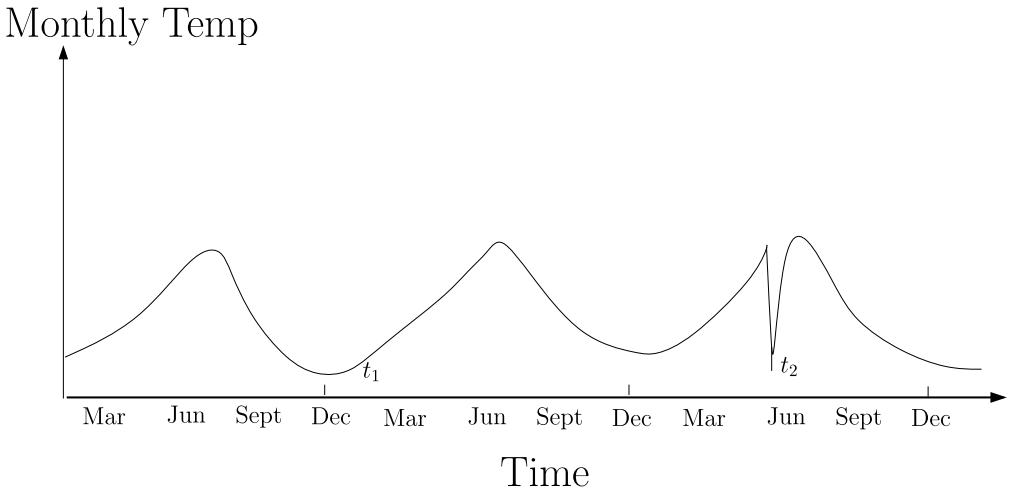
\includegraphics[width=0.7\textwidth]{contextual.png}
		\caption{Example of one contextual anomaly ($t_2$) in a monthly temperature time series dataset. Source: \cite{Kandhari2009}.}
		\label{fig:context_anom}
	\end{figure}
	
	\item \textit{Collective Anomaly}: When a group of data instances of a dataset may not be anomalies by themselves, but when they occur together they can be considered a collective anomaly.
	Figure \ref{fig:collective_anom} illustrates this type of anomaly using a human electrocardiogram output time series: the red values represent a collective anomaly, although that value by itself is not considered an anomaly (despite appearing several times during the dataset just by itself).
	
	\begin{figure}[!ht]
		\centering
		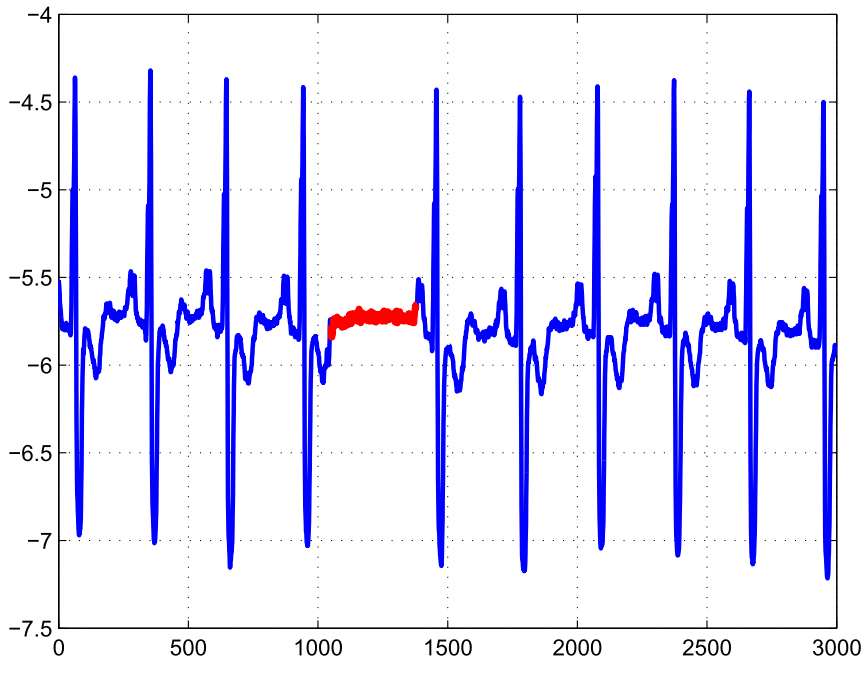
\includegraphics[width=0.6\textwidth]{collective.png}
		\caption{Example of one collective anomaly in a human electrocardiogram output time series dataset. Source:  \cite{Kandhari2009}.}
		\label{fig:collective_anom}
	\end{figure}
	
\end{itemize}

Because of the wide scope of each of these categories, this thesis will only focus on \textit{point anomalies} in the following sections and chapters. Information regarding the techniques capable of detecting contextual and collective anomalies can be found in Kandhari's survey on the topic (\cite{Kandhari2009}).

\subsection{Learning Mode} \label{sec:anomly_learn}

Anomaly Detection techniques can be classified based on the learning mode used:

\begin{itemize}
	\item \textit{Supervised}: Techniques using this learning mode assume that the data is fully labeled as either being \textit{normal} or \textit{anomalous}.
	Therefore, this constitutes a regular supervised learning classification problem. However, it is important to note that in this case the classes are skewed (i.e. there will be have less anomalies in a dataset than \textit{normal} instances).
	
	\item \textit{Semi-supervised}: Techniques using this learning mode assume that the data only contains \textit{normal} examples and try to build a model that can learn the \textit{normal} behavior and identify examples that do not fit in this behavior.
	In the real-world this scenario is very frequent as in many domains it is difficult or expensive to measure anomalies and only \textit{normal} data is available. \textbf{Semi-supervised with both classes exists?}
	
	\item \textit{Unsupervised}: This learning mode does not require labeled data, which makes the techniques based on it more flexible.
\end{itemize}


\subsection{Type of Techniques} \label{sec:anomaly_appr}

The techniques used in Anomaly Detection can be categorized into two groups according to their output \cite{Kandhari2009}:

\begin{itemize}
	\item \textit{Score output:} The techniques with this type of output assign a \textit{score} to each data instance that represents how much the instance can be considered an anomaly. The list of anomalous instances can then be retrieved by using manually defined thresholds on the scores or by marking all the \textit{top-n} instances as \textit{anomalous}.
	
	\item \textit{Label output:} The techniques that output labels resemble regular binary-classifiers in Machine Learning by either classifying a data instance as being \textit{normal} or \textit{anomalous}. These techniques differentiate from the \textit{score} ones as they do not require any type of threshold definition after their application, as the data instance is already labeled as \textit{anomalous} or \textit{normal}.
\end{itemize}

\subsubsection{Classification Based Techniques}

Classification based techniques operate similarly to regular supervised learning classifiers: they train a model based on a set of labeled data and then classify each test data instance as being \textit{normal} or \textit{anomalous}.

One of the disadvantages of this group of techniques is that they require labeled data in the training phase of the model. Depending on the labels available in the training data, the techniques in this group can be subdivided into two types \cite{Kandhari2009}: multi-class and one-class.

%\textbf{TODO: Where does ``isolation forest'' algorithm fit?}

\paragraph{Multi-class Techniques}\mbox{}

Multi-class techniques assume that the training data contains instances belonging to several different \textit{normal} classes and build a classifier that distinguishes each class from the remaining classes. These techniques classify a data instance as being \textit{anomalous} if they cannot classify it as one of the \textit{normal} classes \cite{Kandhari2009}.

Examples of these techniques include certain types of Neural Networks (e.g. Multi Layered Perceptrons, Hopfield Networks), Bayesian Networks, Rule Based techniques, Decision Trees and other binary and multi-class classifiers \cite{Kandhari2009}.

\paragraph{One-class Techniques}\mbox{}

One-class techniques assume that the training data contains instances belonging to only one class -- the \textit{normal} one. The idea behind these techniques when learning the model is to define a decision boundary that isolates the \textit{normal} instances.
This decision boundary can therefore be used to classify new data: data instances that stay inside the decision boundry are are considered \textit{normal} and instances that stay outside the boundary are flagged as anomalies \cite{Kandhari2009}.
These techniques usually operate under the semi-supervised learning method presented in \ref{sec:anomly_learn}.

Examples of these techniques include Replicator Neural Networks \cite{Hawkins}, Support Vector Machines (more specifically One-class SVMs \cite{Sc}) and Rule Based techniques \cite{Kandhari2009}).

\subsubsection{Nearest Neighbor Based Techniques}

Nearest Neighbor based techniques are based on the assumption that \textit{normal} data instances are situated in dense \textit{neighborhoods} of data instances, while \textit{anomalous} data instances situate themselves \textit{far} from other data instances.
The notion of \textit{neighboorhoods} and \textit{far} are employed with similarity/distance metrics that can evaluate how close (or far away) two data instances are.

These techniques can be subdivided into two different groups \cite{Kandhari2009}:
\begin{itemize}
	\item techniques that use the distance of each data instance to its $k^{th}$ nearest neighbor(s) as an anomaly score;
	
	\item techniques that use the concept of relative density of each data instance to compute an anomaly score (which will be detailed in this section).
\end{itemize}

\paragraph{Density Techniques}\mbox{}

The assumption behind the density techniques is that a data instance that belongs to neighborhood with low density (i.e. that contains only a few data instances) is \textit{anomalous}, while the opposite indicates that the instance is \textit{normal}.

\begin{figure}[!ht]
	\centering
	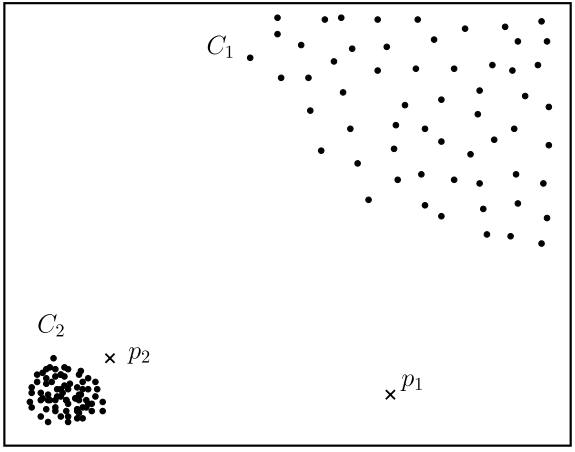
\includegraphics[width=0.6\textwidth]{density_anomalies.png}
	\caption{Example of a 2 dimensional dataset containing regions with different density values. Source: \cite{Kandhari2009}.}
	\label{fig:local_density}
\end{figure}

However, it is important to note that this assumption may not hold if the data has regions with different density values. Figure \ref{fig:local_density} illustrates this example with a 2 dimensional dataset: the distance of each of the instances in cluster $C_1$ to their nearest neighbor is higher than the distance of $p_2$ to its nearest neighbor in cluster $C_2$. Because of this the methods that are based on this assumption would not consider $p_2$ as an \textit{anomalous} instance although visually it is noticeable that this instance is \textit{anomalous} in the given feature space.

In order to overcome this limitation, some techniques within this category compare the density of the data instances to the density of their neighbors. One of the examples of this type of techniques is the LOF (Local Outlier Factor) \cite{Breunig}. Several techniques based on LOF	have been proposed more recently, either to adapt this algorithm to more complex data types or to improve its efficiency. Some examples include COF (Connectivity-based Outlier Factor) \cite{Tang2002}, ODIN (Outlier Detection using In-degree Number) \cite{Hautamaki2004} and LOCI (Local Correlation Integral) \cite{PapadimitriouS.KitagawaH.2003}.

\subsubsection{Clustering Based Techniques}

Clustering is a task in Data Mining in which the goal is to aggregate the data into meaningful or useful groups \cite{Tan2005}. Techniques that capture this idea have been applied to Anomaly Detection, out of which three groups of techniques can be distinguished in the literature based on their assumptions \cite{Kandhari2009}:

\begin{itemize}
	\item \textit{After clustering the data, \textit{normal} data instances belong to one of the clusters formed, while \textit{anomalous} data instances do not belong to any of the clusters}: several clustering algorithms (such as DBSCAN \cite{Ester:1996:DAD:3001460.3001507}) do not force all the data instances to belong to one of the clusters formed. With this particularity of the algorithms and under this assumption, we can consider these data instances as being \textit{anomalous}.
	
	\item \textit{\textit{Normal} data instances situate themselves close to their closest cluster's centroid, while \textit{anomalous} data instances remain far away from any cluster centroid}: these techniques usually use the distance of a data instance to its nearest cluster's centroid as an \textit{anomaly score}. Examples include the use of Self-Organizing Maps (SOM) \cite{Kohonen:1997:SM:261082}.
	It is important to note that if the \textit{anomalous} instances form a cluster by themselves, the techniques under this assumption will not be able to detect them.
	
	\item \textit{\textit{Normal} data instances situate themselves in large and/or dense clusters, while the \textit{anomalous} ones situate themselves in small and/or sparse clusters}: Examples of techniques that operate under this assumption include the FindCBLOF \cite{He:2003:DCL:770340.770389}.
\end{itemize}

\subsubsection{Statistical Techniques}

Statistical techniques operate under the assumption that \textit{normal} data instances occur in high probability regions of a statistical model, while \textit{anomalous} data instances occur in low probability regions \cite{Kandhari2009}.
These techniques consist in building a statistical model of the data, usually using \textit{normal} data instances, similarly to the One-class Classification techniques. However, it is important to note that these techniques have a different assumption from One-class techniques: Statistical techniques are based on statistical models and data instances are considered anomalous if they have a low probability of being generated from the learned model. One-class Classification techniques, however, are based on classification models and in the definition of a decision boundary between instances. In this case, the decision of whether a data instance is \textit{anomalous} or not relies only in the location of the instance within the decision boundary.

The literature distinguishes parametric and non-parametric techniques, which will be detailed in this section.

\paragraph{Parametric Techniques}\mbox{}

Parametric techniques are characterized by making assumptions on the distribution of the data (e.g. assuming it follows a Gaussian distribution or it can be modeled linearly) and build a statistical model of the data, by learning its parameters with \textit{normal} data instances.
The anomaly score of a new data instance can then be calculated from the probability density function of the learned model (if the instance locates itself in a region where the function has a low value it may be considered \textit{anomalous} and vice-versa).
Along with this approach, some techniques also use statistical hypothesis testing to assess if a new data instance is \textit{anomalous} or not.

These parametric techniques can be subdivided into different groups:

\begin{itemize}
	\item \textit{Gaussian Model}: techniques that assume the data distribution is Gaussian. These techniques detect \textit{anomalous} data instances based mostly on thresholds. One simple example of this type of techniques is the box plot rule  \cite{laurikkala2000informal}.
	\item \textit{Regression Model}: techniques that fit a linear model to the data. These techniques consider that a data instance is anomalous if its residual value is above a threshold (i.e. if it is too far away from the model's line). Linear models such as robust regression \cite{leroy1987robust} have been used in these techniques.
	\item \textit{Mixture of Parametric Distributions}: techniques that either model \textit{normal} and \textit{anomalous} data instances as belonging to two different distributions, or by modeling the \textit{normal} data instances as belonging to a mixture of data distributions.
\end{itemize}

\paragraph{Non-parametric Techniques}\mbox{}

Unlike the parametric techniques, the non-parametric approaches do not make any assumptions about the statistical distributions of the data.

These techniques, as well as the parametric ones, can be subdivided into different groups:

\begin{itemize}
	\item \textit{Histogram Based}: these techniques use histograms to maintain a profile of the data (usually only containing \textit{normal} instances). The \textit{anomaly score} of a new data instance is high if it falls in a bin of the histogram with low frequency, and vice-versa.
	\item \textit{Kernel Function Based}: these techniques use kernel functions to estimate the probability distribution function, by using \textit{normal} data instances. The \textit{anomaly score} of a new data instance is high if it falls in a area with low probability, and vice versa.
\end{itemize}

\subsubsection{Information Theoretic Techniques}

Information theoretic techniques analyze the information content of the data with information theory measures (e.g. Kolomogorov Complexity, Entropy) and are based on the assumption that \textit{anomalous} data instances induce irregularities in the information content of the data \cite{Kandhari2009}.

\subsubsection{Spectral Techniques}

Spectral techniques are based on the assumption that \textit{normal} and \textit{anomalous} data instances can distinguished in a lower feature (i.e. in a new	 dataset with a lower number of features) subspace. These techniques often use Principal Component Analysis (PCA) \cite{Jolliffe2002} to project the data into a lower feature space.

\section{Ensemble Learning}\label{sec:ensemble}

%In order to introduce the concept of Ensemble Learning, the following definition (based on the one provided by \textcite{Mendes-Moreira2012}) is proposed:

Based on the definition provided by \textcite{Mendes-Moreira2012}, Ensemble Learning can be defined as: 

\begin{definition}[Ensemble Learning] \label{def:ensemble_learning}
	Ensemble Learning is a process that uses a set of models (ensemble), each of them obtained by applying a learning algorithm to a given problem. This set of models is integrated in some way to obtain the final output.
\end{definition}

It is important to note that this definition is independent of the learning mode, which means that Ensemble Learning can be used for supervised and unsupervised learning \cite{Mendes-Moreira2012}.
Although Ensemble Learning is more frequently applied in supervised learning (classification and regression), it has also been used in clustering \cite{Strehl:2003:CEK:944919.944935}.

However, given the wide scope of these applications, this chapter and the following ones will only focus on classification applications of Ensemble Learning.

Formally, a classification model (or hypothesis) $m = (L, P, \mathcal{D})$ is an application of a learning algorithm $L$, with a set of defined parameters $P$ and trained on a dataset $\mathcal{D} = \{(x_n, y_n), n = 1, \dots, N\ \}$, where $x_n$ represents the feature values of the \textit{n}th instance and $y_n$ the class value of the \textit{n}th instance.
Given a data instance $x_i$ from a dataset $\mathcal{D}$, $m(x_i)$ is the prediction of the class value of $x_i$ made by model $m$.

Therefore, an ensemble $E = \{m_i, i = 1, \dots, M \}$ can be defined as a set of $M$ models, where $E(x_i) = g(m_1, \dots, m_M)$ corresponds to the prediction of the class value of $x_i$ by the ensemble $E$. This prediction is made using an aggregation function $g$ which combines the predictions from the $M$ models of the ensemble, $m_1(x_i), m_2(x_i), \ldots, m_M(x_i)$.
%It is important to mention that this definition is recursive, as an ensemble can also be considered a model in another ensemble.

%Formally, let $m$ be a model obtained by applying a learning algorithm $A$ with parameters $P$ to a dataset $D$, and $E = {m_1, ..., m_n}$ be an ensemble of $n$ models. Given a new data instance $d$, let $R = {r_1, ..., r_n}$ be the outcomes 

%Formally, a model (or hypothesis) $m = (L, P, \mathcal{D})$ is an instantiation of a learning algorithm $L$, with a set of defined parameters $P$ and trained using on dataset $\mathcal{D}$.
%Let $x_i$ \textbf{DEFINIR O QUE É DATA INSTANCE -  ver paper Stacked Generalization: when does it work?} be a data instance, $m(x_i)$ corresponds to the prediction of $x_i$ from a model $m$.
%It is important to note that the definition of model in unsupervised learning implies $\mathcal{D} = \emptyset$, since there is no training phase.

%Therefore, an ensemble $E = \{m_1, \dots, m_n \}$ can be defined as a set of $n$ models, where $E(x_i)$ corresponds to the prediction of $x_i$ by the ensemble $E$.
%It is important to mention that this definition is recursive, as an ensemble can also be considered a model in another ensemble.
The different ways in which the set of models can obtained and then integrated to obtain a final output will be discussed further in this section. 

%In this context, it is also important to provide the following definition of \textit{model}:

%\begin{definition}[Model]
%	A model (or hypothesis) corresponds to the instantiation of a learning algorithm to a specific problem (which can be represented by dataset).
%\end{definition}

It is also important to refer that approaches with \textit{Multiple Models} or \textit{Multiple Learners} presented sometimes throughout the literature refer to the same concept presented in this section \cite{Mendes-Moreira2012}.

\textcite{Dietterich1990} presents three reasons why Ensemble Learning can lead to better results:

\begin{itemize}
	\item Applying a learning algorithm to a specific problem can be interpreted as searching for the best model for this problem (the one that is considered the \textit{best} according to a predefined metric) within a space of possible models $H$. When the dataset provided is too small compared to the space $H$, several models can be equally considered the \textit{best}. By building an ensemble of this set of models, it is possible to obtain a new model that may generalize better to new data.
	
	\item Some learning algorithms generate models for a specific problem by performing an optimization process over an error function, which can get stuck at a local minimum. This is the case, for example, of neural network algorithms. By building an ensemble of different models (obtained by starting this optimization at a different starting points), it is possible to obtain a model that is closer to the global minimum.
	
	\item Given a specific problem, a learning algorithm works by instantiating a model the mimics the underlying process that can explain this problem (which will be represented by $f$). However, some learning algorithms (e.g. linear algorithms) may not have a model space $H$ large enough to contain a model that can represent $f$ accurately. By building an ensemble of different models and combining their outputs, it may be possible to expand the model space $H$ and have a better approximation of $f$.
\end{itemize}

\textcite{hansen1990neural} however state that there are two necessary (and sufficient) conditions for an ensemble of models to be more accurate than any of individual models that belong to it:

\begin{itemize}
	\item Each of the models that compose the ensemble must be \textit{accurate}, which according to the author is to be better than random guessing.
	
	\item The ensemble of models should be \textit{diverse} (i.e. the outputs of the models should be uncorrelated to each other).
\end{itemize}

%\textbf{Introduce dimensions of taxonomy}

\textcite{Mendes-Moreira2012} proposes a three phases to be considered when using Ensemble Learning, which will be detailed in this section. \textbf{ESQUEMA AQUI}

%\begin{figure}[th!]
%	\centering
%	\includegraphics[width=0.7\textwidth]{figures/ensemble_learning_process}
%	\caption{Illustration of the three-process in Ensemble Learning. Based on \cite{Mendes-Moreira2012}.}
%	\label{fig:ensemblelearningprocess}
%\end{figure}

\subsection{Ensemble Generation}\label{sec:ens_gen}

The initial step in the process of Ensemble Learning is to generate an ensemble of models. We are interested in generating a set of models $\mathcal{M}_0 = \{ m_i, i = 1, \dots, M_0 \}$.

Ensembles can be of two different types \cite{Mendes-Moreira2012}:

\begin{itemize}
	\item \textit{Homogeneous}: when the set of models are generated by the same learning algorithm (e.g. tuned with different parameter settings). Most of the research work in Ensemble Learning is conducted with this type of ensembles \cite{Mendes-Moreira2012}.
	\item \textit{Heterogeneous}: when the set of models are generated by different learning algorithms. This type of ensembles may have more diversity between models than the homogeneous type, if nature of the learning algorithms is diverse enough \cite{Mendes-Moreira2012}.
\end{itemize}

It is interesting to note that homogeneous ensembles can be used in heterogeneous ensembles, given the recursive definition of ensemble.

A possible methodology that can be followed is the \textit{overproduce-and-choose} approach.
In this methodology a high number of models are generated in the ensemble generation phase (``overproduce''), leaving the task of selecting the best models to the pruning phase (``choose'').	

\textcite{Mendes-Moreira2012} presents different ways to produce different models in both homogeneous and heterogeneous ensembles, which will be detailed in this section.

\subsubsection{Data Manipulation Approaches}

In the definition of a model $m = (L, P, \mathcal{D})$, these approaches perform changes in the dataset $\mathcal{D}$ used to train the learning algorithm $L$. The same learning algorithm trained with different datasets will result in different models (which may or may not be diverse in-between, depending on the stability of the algorithm and its sensibility to the training dataset).

\paragraph{Subsampling from the Training Set}\mbox{}

This type of approach generates different models using different subsamples of the same dataset.

One of the most popular approaches is $bagging$ (bootstrap aggregating), which generates $k$ subsamples of a dataset $\mathcal{D}$.
These subsamples are made with replacement (a subsample can contain a data instance more than once).
A model is then trained with each of the $k$ subsamples generated, generating $k$ different models.

\paragraph{Manipulating the Input Features}\mbox{}

This type of approach can be divided in two subtypes:

\begin{itemize}
	\item \textit{Feature Selection}: 
		A feature selection process is performed on the dataset, in order to generate different datasets (each one with a different subset of features).
		One example of this approach is the \textit{random subspace} method \cite{ho1998random} (which chooses randomly feature subsets).
		
	\item \textit{Feature Transformation}:
		A transformation is conducted on the features' original values, in order to generate different datasets with different features.
		One example is the \textit{input smearing} approach \cite{Frank2006} that adds Gaussian \textit{noise} to each numeric feature.
\end{itemize}

\textit{Rotation forests} (proposed by \textcite{1677518}) incorporates both feature selection and transformation processes. First, this method selects different $k$ disjoint subsamples of features. Then, for every subsample, PCA is performed to project the feature space into a new one, where the new features correspond to linear combinations of the original ones.

\subsubsection{Model Generation Manipulation}

This type of approaches manipulates the learning algorithm's parameters or learning conditions.

\paragraph{Manipulating the Parameter Set}\mbox{}

Manipulating the parameter set of a learning algorithm is a possibility to generate different models, either by iterating by ranges of possible values (Grid Search \cite{hsu2003practical}) or using a Random Search \cite{bergstra2012random}.

\paragraph{Manipulating the Induction Process}\mbox{}

In order to to obtain a model $m$ from a learning algorithm $L$ on a dataset $\mathcal{D}$ it is necessary to perform an \textit{induction}. This type of approaches try to change the way in which the model is generated, allowing the generation of models under different induction conditions.
One of the most common approaches is to change the error function in optimization-based learning algorithms (such as neural networks).

\paragraph{Manipulating the Generated Model}\mbox{}

This type of approaches performs adjustments on an already generated model, leading to different models.
One known approach is to change a Classification Association Rules (CARs) model by subsampling the model's set of rules $n$ times, generating $n$ models with different sets of rules. 
	
\subsection{Ensemble Pruning}

The generation of an ensemble in the previous phase, although might guarantee a wide diversity of models, it does not guarantee that the smallest ensemble possible with maximum accuracy was obtained. Several of the models may also have very correlated outputs, which do not add any extra knowledge to the final prediction.
Also, since some of the approaches for generating ensembles involve randomness, there is no guarantee all the models in the ensemble will contribute positively to the final prediction.

Therefore the goal of Ensemble Pruning is to: improve the predictive accuracy of the ensemble and reduce the ``cost'' of the ensemble (since an ensemble with a higher number of models will be more computationally costly to use).

Ensemble Pruning consists in selecting a subset $\mathcal{M}$ with $M$ models of the set of models generated in the previous step.
This phase corresponds to the ``choose'' step of the \textit{overproduce-and-choose} methodology presented in section \ref{sec:ens_gen}. Therefore, $\mathcal{M}$ follows the succeeding property:

\begin{equation}
\mathcal{M} \subseteq \mathcal{M}_0
\end{equation}

A possible heuristic to choose the models can be, for example, a combination of diversity and/or accuracy. Several metrics suitable for measuring diversity and accuracy will be discussed further in this chapter, in section \textbf{PREENCHER COM A SECTION}.

\textcite{Mendes-Moreira2012} proposes two types of approaches for conducting Ensemble Pruning, which will be detailed in this section.

\subsubsection{Partition-Based Approaches}

The main idea of partition-based approaches is to cluster the models into several groups. This could be done, for example, with the clustering algorithm k-means, in order to obtain a set of clusters of similar models.
Afterwards, one or more representative models from each group are chosen to constitute the pruned ensemble.

\subsubsection{Search-Based Approaches}

Search-based approaches can divided in three different types:

\begin{itemize}
	\item \textit{Exponential Search Approaches}: Exponential Search Approaches search the complete search space of possible models to be included from $\mathcal{M}_0$. This search space has $2^{M_0} - 1$ possible subsets of models and the search for the optimal subset is an NP-complete problem.
	
	\item \textit{Randomized Search Approaches}: Randomized Search Approaches perform a heuristic search in the search space (e.g. using evolutionary algorithms). Approaches such as genetic algorithms, tabu search and population-based incremental learning have been used in previous works \cite{Ruta2001}.
	
	\item \textit{Sequential Search Approaches}: Sequential Search Approaches perform a search by iteratively adding and/or removing a model from subset to maximize some criteria.
	This can be done using using \textit{Forward Subset Selection}, \textit{Backward Subset Selection} or a combination of both.
	In \textit{Forward Subset Selection}, the search starts with am empty ensemble and models are iteratively added.
	In the case of \textit{Backward Subset Selection}, the search starts with all the possible models generated in the ensemble and they iteratively removed.
\end{itemize}

\subsection{Ensemble Integration}

The final step in Ensemble Learning is the combination of the predictions from the models in the ensemble.

In classification, the most popular approaches to combine models can be divided into two categories: combination-based approaches and model-based approaches.

\subsubsection{Combination-based Approaches}

Combination-based approaches are based on combination rules of the class values outputted by the models in the ensemble.
First it is important to define the decision of the $i^{th}$ model (referred in section \ref{sec:ensemble} as \textit{class value}) as $d_{i,c} \in \{ 0,1 \}, i = 1, \dots, M$ and $c = 1, \dots, C$, where $M$ is the number of models in the ensemble (as defined previously in section \ref{sec:ensemble}) and $C$ is the number of classes.
If the $i^{th}$ model outputs class $c$, then $d_{i,c} = 1$ and 0 otherwise.

\paragraph{Majority Voting}\mbox{}

Majority Voting has three different subtypes, in which the ensemble output corresponds to the class in which all classifiers agree (\textit{unanimous voting}), the class predicted by at least one more than half the number of classifiers (\textit{simple majority}) or the class predicted by the majority  of the classifiers, even if it is predicted by less than half of the number of classifiers (\textit{plurality voting}) \cite{Polikar2012a}.

The Majority Voting approach (unless specified otherwise) usual refers to \textit{plurality voting} \cite{Polikar2012a} and the decision of which class value to output can be defined as follows: 

\begin{equation}
\max_c \sum_{i = 1}^{M} d_{i,c}
\end{equation}

\paragraph{Weighted Majority Voting}\mbox{}

If it is known that some of the models are more likely to make correct predictions than others, weighting the decisions of the models can improve the performance of the Majority Voting approach \cite{Polikar2012a}.
In this case, models with higher performance would have a bigger weight assigned and models with a worse performance otherwise.
We define the weight of a model $m_i$ as $w_i$.
These weights usually are normalized so that:

\begin{equation}
w_i \in [0, 1] \ \wedge \ \sum_{c = 1}^{C} w_{i} = 1, \ \forall i \in M
\end{equation}

In this case, the decision of the class output is defined as follows:

\begin{equation}
\max_c \sum_{i = 1}^{M} w_i \cdot d_{i,c}
\end{equation}

A estimation of the weights could be performed by estimating the models' generalization performance in a separate validation set.

\paragraph{Borda Count}\mbox{}

The Board Count method assumes that each model is capable of ranking its support to each class $c$ and takes this into consideration \cite{Polikar2012a}. This method can be particularly useful in multi-class problems where $C$ takes a considerable value.

For each model $m_i$, each class $c$ receives $C-r$ votes being $r$ the position of $c$ in the ranking belonging to model $m_i$.
For example, if $C = 4$ and the class 1 is ranked $3^{rd}$ by model $m_1$ (meaning that model $m_1$ picked class 1 as being the third most probable), then class 1 will receive $4-3 = 1$ votes.
This procedure is then executed for each model and possible class value, the results are added up and the class with higher number of votes is chosen.

\subsubsection{Model-based Approaches}

Throughout the literature in Ensemble Learning, several more complex methods of prediction combinations are described \cite{Polikar2012a}.
Some of these can be considered model-based, in the sense that there is a training phase of an algorithm that ``learns'' how to combine the several models in the ensemble.
We will describe briefly two possible approaches in this section.

\paragraph{Stacked Generalization}\mbox{}

\begin{figure}[ht!]
	\centering
	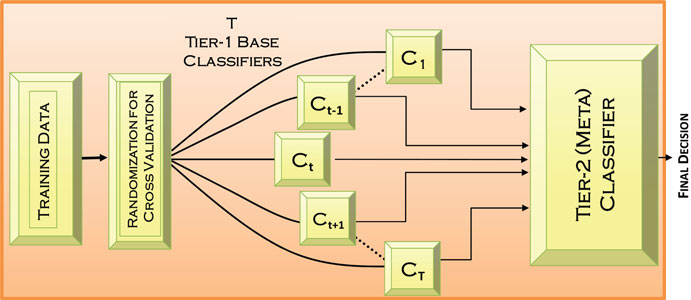
\includegraphics[width=0.8\textwidth]{figures/stacking}
	\caption{Scheme of the Stacked Generalization approach. Source: \cite{Polikar2012a}.}
	\label{fig:stacking}
\end{figure}

Stacked Generalization (also known as Stacking) is an Ensemble Learning method in which the predictions of the models are combined using another model (also known as a \textit{meta-classifier}) \cite{Polikar2012a}. In order to do so, a new dataset is generated using the prediction outputs of the models belonging to the ensemble.
This new dataset is then used to generate another model (the \textit{meta-classifier}). This mechanism is illustrated in figure \ref{fig:stacking}

This approach can be seen as an extension of the Weighted Majority Voting.
However, unlike this method, the impact of each model in the final decision is not translated into a single value.
Stacking allows to determine which models are likely to be accurate in several parts of a dataset's feature space, since certain models may be more ``specialized'' in predicting correctly certain data instances.
In this case the predictions of these models for these data instances will have a higher ``weight'' and the remaining models a lower one.

Since this approach is the main focus of this dissertation, we will focus on it in chapter \textbf{METER CHAPTER}.

\paragraph{Mixture of Experts}\mbox{}

\begin{figure}[ht!]
	\centering
	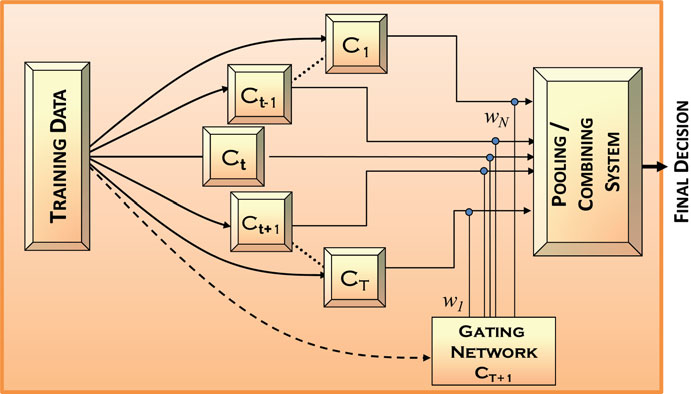
\includegraphics[width=0.8\textwidth]{figures/mixture_models}
	\caption{Scheme of the Mixture of Experts approach. Source: \cite{Polikar2012a}.}
	\label{fig:mixture}
\end{figure}

As the name reflects, the Mixture of Experts approach assumes certain individual models may be \textit{experts} in predicting the class value for certain data instances but more inaccurate for the remaining ones in the dataset. This background idea is very similar to the one behind Stacking, in which weights are assigned to each model of the ensemble reflecting its accuracy in certain parts of the dataset's feature set

However, these weights are not determined by a new model but by a \textit{gating network} (as illustrated in \ref{fig:mixture}).
This gating network is trained using the expectation-maximization (EM) algorithm on the original dataset.



%\textcite{Dietterich1990} defines several methodologies that can be used to generate homogeneous ensembles:

%\begin{itemize}
%	\item \textit{Manipulating the Training set:} Several instances of a specific learning algorithm are trained on a set of different training sets, generating different models. This methodology is usually applied when the learning algorithm is \textit{unstable} (i.e. if the outputs of the algorithm change with little changes on the training set): examples of \textit{unstable} learning algorithms are decision trees and neural networks, while linear regression and k-nearest neighbors are considered \textit{stable} algorithms. Bootstrap Aggregation \cite{Breiman1996} (also known as Bagging) and AdaBoost \cite{freund1995desicion} are examples of ensemble methods that use this methodology.
	
%	\item \textit{Manipulating the Input Features:} Several instances of a specific learning model are trained with the same training set, but with different sets of features, generating different models. This methodology has good results when some of the original input features are redundant.
	
%	\item \textit{Injecting Randomness within Model Generation:} Several instances of a specific learning algorithm are randomly tuned within different parameters, generating different models.
%\end{itemize}

%After generating an \textit{ensemble} of models, their output has to be combined in order to integrate them into a single decision.

\section{Ensemble Learning Applications in Anomaly Detection}

\textbf{Falar de Ensembles Supervisionados e não-supervisionados (muito brevemente)}

%-- Ways to combine outputs

%In order to better understand the different approaches within the field Ensemble Learning, a taxonomy proposed by \textcite{Re2011} will be presented in this section (based on the ones proposed by \textcite{Valentini:2002:ELM:645961.674073} and \textcite{Kuncheva:2004:CPC:975251}).

%\textbf{TODO: table}

\subsection{Supervised Approaches}

\subsection{Unsupervised Approaches}

Vast majority of the literature

Categorization by component (model) independence

Sequential ensembles (estes tendem a ser menos explorados, estão mais guiados para problemas de classificação), independent ensembles

Categorization by constituent components (models)

Posso falar da relação disto com o subspacing: Just as ensemble analysis works well in cases in which different algorithms work better on different subsets of points, high-dimensional outlier detection works best in cases where different subspaces are relevant to different sets of points. Therefore, by using ensemble components to explore different subsets of dimensions, one is often able to combine the results of these different exploratory base detectors to create stable and accurate results. (livro do Aggarwal)

There are two key design choices in the construction of an ensemble method:
Choice of base detector:



Methodology for score normalization and combination:

For example, a k-nearest neighbor algorithm would typically output scores on a different scale than the LOF algorithm. Similarly, an EM-algorithm might output fit values in which outliers would tend to have lower scores. On the other hand, most algorithms assume the opposite convention. Therefore, it is important to normalize scores, so that one can meaningfully combine various algorithms without inadvertently over-weighting one of the algorithms.

For the cases when the outliers have bigger or smaller scores, a solution is to flip the sign of the scores.

Then can then be normalized:
- Range based scaling - between 0 and 1
- Standardization - more reliable. Note that standardization uses the assumption that the 1-dimensional scores follow a normal distribution. Although this assumption is almost never true, this type of normalization can often provide reasonably robust results.

Também é possível converter para probabilidades com o EM algorithm.

Combine the scores:
- Averaging
- Maximum (reduz bias mas aumenta a variancia)

\textbf{**Variance reducing ensembles**}

\textbf{Parametric Ensembles}
The most straightforward application of variance reduction is that of addressing the issue of parameter choice in outlier detection algorithms.

A typical ensemble approach [31] is to use a range of different values of k, and then average the scores. Although the overall performance might not be as good as that of using the best value of k, it is usually better than the median performance over the different values of k that are tested. The resulting detector has reduced variance than that of a detector that selects one of these reasonable choices of parameters randomly.

It is noteworthy that this particular view of variance reduction is over different randomized instantiations of the base detector rather than over different randomized draws of the training data from the base distribution. Therefore, such an approach reduces model-centric variance.

In general, methods like clustering and histograms are so sensitive to the choice of parameters that it makes sense to use them only in this type of ensemble-centric setting.

\textbf{Randomized Detector Averaging}

Many outlier detection models are inherently randomized because they depend on the use of randomly chosen initialization points. For example, if a data point is scored using its distance to the closest centroid of a k-means algorithm, the scores may vary significantly from one execution to the next because of the effect of the initialization point. Therefore, in all such cases, it is extremely important to run the model multiple tries and average the scores in order to reduce the effect of variance on modeling accuracy.

\textbf{Feature Bagging}

Ver a ideia no livro

\section{Evaluation Metrics}

\subsection{Model Performance}
cena

\subsection{Model Diversity in an Ensemble}
cena2

\section{Datasets for Evaluation}

Falar do estudo feito sobre datasets para unsupervised anomaly detection

\section{Summary}

Resumo do chapter


%we will only focus in unsupervised learning approaches

%\section{Summary}